\documentclass[11pt]{article}
\usepackage{color}
\usepackage{graphicx}
\usepackage{amsmath,amsthm,amssymb,multirow,paralist}
\usepackage[margin=0.8in]{geometry}
\usepackage{hyperref}

\begin{document}

\begin{center}
{\Large \textbf{COM S 474/574: Introduction to Machine Learning}\\Homework \#3}\\

\linethickness{1mm}\line(1,0){498}

\begin{enumerate}
\item Please put required code files and report into a
compressed file ``HW\#\_FirstName\_LastName.zip''
\item Unlimited number of submissions are
allowed on Canvas and the latest one will be graded.
\item {\color{red} No later submission is accepted.}
\item Please read and follow submission instructions. No exception
will be made to accommodate incorrectly submitted files/reports.
\item All students are required to typeset their reports using
latex. Overleaf
(\url{https://www.overleaf.com/learn/latex/Tutorials}) can be a
good start.
\end{enumerate}

\linethickness{1mm}\line(1,0){498}

\end{center}

%%%%%%%%%%%%%%%%%%%%%%%%%%%%%%%%%%%%%%%%%%%%%%%%%%%%%%%%%%%%%%%%%%%%%%%%%%%%%%%

%%%%%%%%%%%%%%%%%%%%%%%%%%%%%%%%%%%%%%%%%%%%%%%%%%%%%%%%%%%%%%%%%%%%%%%%%%%%%%%


\begin{enumerate}

\item (30 points) You are provided with a training set of
examples (see Figure~\ref{fig:tree}). Which feature will you pick
first to split the data as per the ID3 decision tree learning
algorithm? Show all your work: compute the information gain for
all the four attributes and pick the best one.

\begin{figure*}[ht]\label{fig:tree}
\begin{center}
    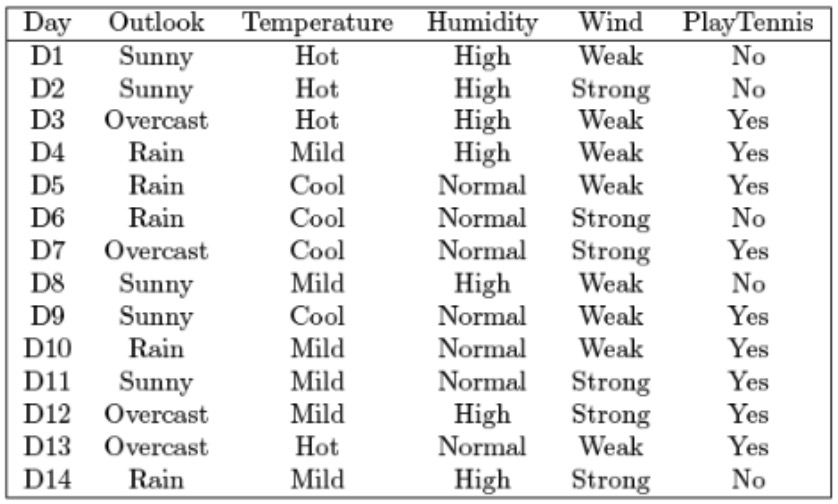
\includegraphics[width=0.6\textwidth]{FIG/tree.jpg}
    \caption{Table with training examples. Each row corresponds
    to a single training example. There are four features,
    namely, outlook, temperature, humidity, and wind.
    ``PlayTennis'' is the class label.}
\end{center}
\end{figure*}

\item (20 points) \textbf{ Principal Components Analysis}
    
    Given three data points: $(-1, -1), (0,0), (1,1)$.

    \begin{enumerate}
        \item (10 points) Show the first Principal Component
        (actual vector) without using Eigendecomposition. Justify
        your answer.

        
        \item (10 points) If use the $1^{st}$ principle component
        to transform the data into 1-d space. What are the new
        data?


\end{enumerate}

\item (50 points) \textbf{Principal Component Analysis:}
    
    In this homework, you will apply the principal component
    analysis to a collection of handwritten digit images from the
    USPS dataset. The USPS dataset is in the ``data'' folder:
    USPS.mat. The starting code is in the ``code'' folder. The
    whole data has already been loaded into the matrix $A$. The
    matrix $A$ has shape $3000\times 256$ and contains all the
    images. Each row in $A$ corresponds to a handwritten digit
    image (between 0 and 9) with size $16\times 16$. You are
    expected to implement your solution based on the given codes.
    The only file you need to modify is the ``solution.py'' file.
    You can test your solution by running the ``main.py'' file.
    
    \begin{enumerate}
    \item (20 points) In PCA, we obtain a projection matrix or
    reduce matrix $\boldsymbol U \in \mathbb{R}^{d\times p}$.
    Based on $\boldsymbol U$, we project the original centered
    data $\boldsymbol{\bar{X}} \in \mathbb{R}^{d\times n}$ into
    reduced data $\boldsymbol{Z} \in \mathbb{R}^{p\times n}$.
    Complete the \emph{\textbf{\_do\_pca()}} method. You only
    need to center the data instead of applying mean
    normalization. Your code will be tested on $p$ = 10, 50, 100,
    200, total four different numbers of the principal
    components.
    
    \item (10 points) Based on the projection matrix $\boldsymbol
    U$ and reduce data $\boldsymbol{Z}$, we can reconstruct the
    original data  $\boldsymbol{{X}'}$ by $\boldsymbol{U}
    \boldsymbol{Z}$ and adding back the original means. Here you
    need to  Complete the \emph{\textbf{reconstruction()}} method
    to reconstruct the reduced data.
    
    \item (10 points) Based on the reconstructed data
    $\boldsymbol{\bar{X}'}$, we can compute measure the
    reconstruction error by $||\boldsymbol X -
    \boldsymbol{{X}'}||^2_F$. Complete the
    \emph{\textbf{reconstruct\_error()}} function to measuring
    the reconstruction error.
    
    \item (10 points) Run ``main.py'' to see the reconstruction
    results and summarize your observations from the results into
    a short report. When you run the ``main.py'' file, a subset
    (the first two) of the reconstructed images based on p = 10,
    50, 100, 200 principal components will be automatically saved
    on the ``code'' folder. Please attach these images into your
    report also.
    \end{enumerate}
    
    
    \textbf{Note:}You are NOT supposed to use existing PCA libraries; instead, you should write your own PCA. Please read the ``Readme.txt'' file carefully before you start this assignment.

\end{enumerate}

\end{document}
